\section{Real-world Application: the Monty Knowledge Base}
\label{sec: swisscom}

\subsection{Motivation}

Knowledge graphs as a data structure have witnessed numerous applications in a diverse range: journalism, biomedicine, social networks, network security, and, recently, telecommunication. Thus, like many other companies, Swisscom (Switzerland) AG has started building and maintaining its knowledge graph for internal use in the last few years. The end goals include the possibility to analyse telecommunication infrastructure in detail, predict and diagnose possible communication defects that may arise, speed up retrieving customer support information, and many other applications.

Previous research work in the company presented an approach that addressed these prediction challenges; however, experiments showed weak generalization performance for other data sources. Thus, the goal of the study in this section was to present a detailed network-science-based analysis of the properties of this knowledge graph, and more importantly, in what manner they differ most from the properties of publicly available knowledge graph data that can be used for evaluating graph models. The completed results from this study allowed us to perfect the COINs model and apply it successfully to Swisscom's \enquote{Monty} knowledge base. 

Specifically, in this section, we will present a detailed descriptive and comparative knowledge graph analysis methodology that was applied to the company's data, though it is general and detailed so as to be operationalized for broader research purposes. We dissect a knowledge graph with five classes of network science measuring techniques and utilize one-sample goodness of fit and two-sample distribution comparison statistical tests to quantitatively analyze the obtained measures. Before concluding, we present the final link prediction and query answering results on the Monty data. We believe the methodology presented in the following pages has practical research value for constructing all knowledge graph reports. 

\subsection{Related work}
\label{sec:related_work}

As we introduced in Chapter \ref{chp: background}, the field of \emph{network science} studies methods for analysing specific properties of graph-structured data in order to obtain insight that might be useful for building a predictive model of the target graph/network. The book by \cite{barabasi_network_2016} is a very good introduction to this scientific field, and we adopt the definitions of most graph-related concepts and metrics from this source. Though more dedicated to a random graph theory view of networks, \cite{lewis_network_2011} also details classical tools.

In \cite{pinheiro_social_2011}, one can find recommended network science methods for the application of telecom graphs, viewed from the perspective of social networks between customers. On the other hand, we distinguish the experiments by \cite{kostic_social_2020} as the only recent work found directly applying empirically estimated features from an (again customer-level) telecom network for the churn prediction problem. Though our data structure and task differ, the authors, alike \cite{pinheiro_social_2011}, support the utility of network connectivity, network clustering, and node importance metrics for the telecom use case, techniques we also employ. We thus hope our study will also similarly empirically motivate and validate similar future work.

\subsection{Methodology}
\label{sec:methodology_swisscom}

As previously introduced, the goal of this project is to dissect and demystify an enormous knowledge graph by producing a detailed report of its properties represented through network features obtained from a thorough unsupervised analysis. Inspired by both classical network science theory and recently proposed methods, we compute 5 classes of network features to form the set of descriptors. For a statistical-test-based comparison between the features as the representation of a graph, we execute the same descriptive procedure for a set of selected public datasets as well. We elaborate on the computational process of the 5 feature classes and statistical comparison in the rest of this section.

\subsubsection{Heterogeneity}

Swisscom's internal knowledge graph is confirmed to be a directed AMHEN. Around 10-50 possible labels for both entities and relations are available. 
 
The presence of type labels for nodes and edges separates AMHENs from simple directed multiplex graphs. To quantify this heterogeneity in detail, we empirically measure the distribution of node types, the distribution of relation types, and the distribution of (head type, relation type, tail type) triplets through appearance frequencies. Note that although the first two distributions can be viewed as marginals of the third, they offer the option for the separation of label distribution comparison. 

To quantify heterogeneity while also acknowledging its dependence on graph structure, \cite{newman_mixing_2003} proposes the \emph{nominal assortativity} scalar metric for node types. The value is alike a correlation coefficient, negative values indicate frequently changing node types across graph paths, positive values indicate that node types are instead more likely to be preserved across paths, while 0 would be obtained from a uniformly-random label assignment.

\subsubsection{Connectivity}

Quantifying global and local connectivity in relational models is one of the main goals of network science. Connectivity metrics attempt to measure the reachability and neighbourhood sizes of nodes, transitivity of relations, etc. For this work, we considered classically:
\begin{itemize}
    \item Edge density, defined as the ratio of the number of edges to the total possible edges;
    \item Node in-degree and out-degree distributions as value appearance frequencies;
    \item Average path length and graph diameter (maximum path length);
    \item Sizes of weak (undirected) and strong (directed) connected components;
    \item Clustering coefficient for each node, as well as average clustering.
\end{itemize}

Beyond this classical connectivity report, we also compute two scalar metrics quantifying the distribution of connectivity across the graph, used in state-of-the-art generative graph model research for evaluation through similar graph comparison \cite{krawczuk_gg-gan_2020}. Namely, we implement \emph{degree assortativity proposed} by \cite{newman_mixing_2003}, as well as the \emph{algebraic connectivity} metric, defined as the second-smallest eigenvalue of the graph Laplacian matrix \cite{chung_spectral_1996}.

\subsubsection{Importance}

The field of network science also researches how to quantify important/influential entities in a network, by computing some measurable score for vertices according to an underlying theory.

The classical centrality measures are one such class of scores, and for this work, we utilize closeness and betweenness centralities, defining important nodes as those with high reachability or high utility in shortest paths, respectively.

Due to the extreme relevance of the node importance problem, more complex and very prominent algorithms exist, and for this work, we utilize the hub and authority scores of the HITS algorithm \cite{kleinberg_authoritative_1999} as well as PageRank \cite{brin_anatomy_1998}.

\subsubsection{Subgraphing}

Given the sheer scale of Swisscom's internal knowledge graph (millions of entities), there is a non-negligible probability of noise and irrelevant information in a graph of that size. Thus, unlike the public data sources, whose size permits a direct computation of metrics belonging to the above three introduced classes, it was decided to structure the analysis pipeline according to domain relevance and applicability. Specifically, we obtain a covering of Swisscom's internal graph through bootstrap sampling of subgraphs. 

The procedure is graphically summarized in Figure \ref{fig:subgraphing}, while the details are as follows. The full knowledge graph is stored in the form of a Neo4j$\textsuperscript{\textregistered}$ graph-NoSQL database. Domain-relevant queries are first used to extract subgraphs describing part of the networking infrastructure that provides Swisscom services to a customer. When all of the extracted subgraphs (either rooted at customer organizations or customer sites) are merged with a simple union operation, the scale of the covering will at most be equal to the original scale of the graph, as we would prefer.

\begin{figure}[H]
\centering
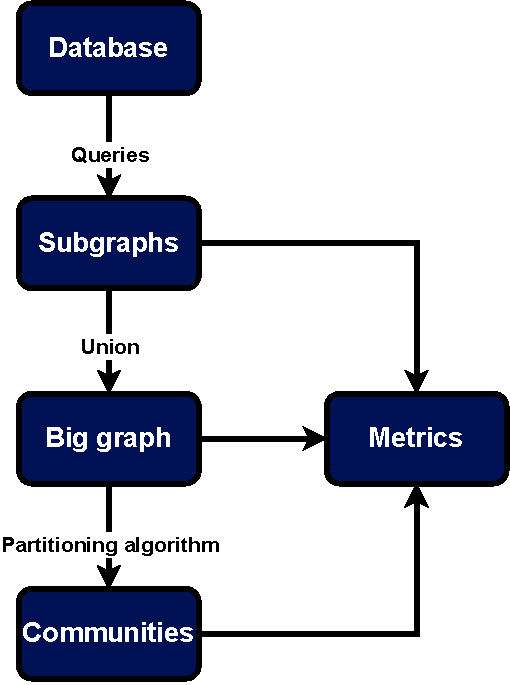
\includegraphics[width=0.35\columnwidth]{figures/swisscom/subgraphing.pdf}
\caption[Monty subgraphing pipeline.]{Monty subgraphing pipeline.}
\label{fig:subgraphing}
\end{figure}

To achieve scalability, the previously developed predictive model utilizes subgraph-based locality of entities and relations to reduce the underlying computational complexity. In order for this approach not to sacrifice prediction accuracy, the subgraphs ideally should be both \emph{representative} samples of the full data, while also sufficiently \emph{informative} such that the subgraph assignment has meaning itself. To help balance these two desirable properties, one can guide the design of the query-based subgraphing by comparing its result to that of a dedicated graph-structure-based partitioning algorithm from the field of community detection. For extracting disjoint communities from the aggregate graph, we employ the state-of-the-art Leiden algorithm \cite{traag_louvain_2019} for Monty too, while EgoNetSplitter \cite{epasto_ego-splitting_2017} can efficiently compute a community covering with overlaps.

Due to this design of our subgraphing analysis, we are able to analyze the data from both a macroscopic and microscopic level, by computing the metrics for the big graph, as well as for each subgraph, community, overlap between subgraphs, or overlap between EgoNetSplitter communities, yielding valuable diagnostic opportunities.

The community detection procedures yield useful metrics themselves; we focus on the community size distribution for both the disjoint and overlapping cases, the size distribution of overlapping regions, as well as the Leiden modularity measure of the disjoint partitioning.

Regarding analyzing the subgraph structure of a network, a popular approach is also to estimate the frequencies of all possible tiny non-isomorphic subgraphs, called \emph{motifs}. For this work, we enumerate all of the possible 3 and 4-node directed subgraphs to use as motifs and use the Efficient Sampling Algorithm (ESA), proposed by \cite{kashtan_efficient_2004}, to estimate their frequency distribution.  

\subsubsection{Summarization}

The field of graph summarization \cite{liu_graph_2019}, gaining traction in recent years, focuses on obtaining graph \emph{summaries} in order to reduce data volume and storage, speed up graph algorithms and queries, support interactive graph analysis, and eliminate noise. The notion of a graph summary is not well defined; summaries are application dependent and can be defined with respect to various goals, performing data compression in addition to preserving specific structural patterns, preserving answers to graph queries, or maintaining the distributions of graph properties. 

The KGist algorithm \cite{belth_what_2020} was first considered for the purpose of this study. The method is based on bit-compression techniques, discovering the optimal set of association rules between labels that balance their total description length with the number of relations in the knowledge graph they explain. These metrics are also convenient for comparison of the summary to those of the public graphs.

As preserving query answers and obtaining a summary in the form of a knowledge graph is also desirable for our application, we additionally implement a labeled-graph variation of the graph de-densification algorithm by \cite{maccioni_scalable_2016}. Using node degrees, the method discovers densely-connected pairs of node sets and rewires these locally-dense regions in a manner that would sparsify the graph while preserving the query result depending on those nodes. The final achieved compression ratio is a useful metric to report. 

Due to the query-relevant nature of our knowledge graphs, we deemed it also profitable to compare datasets w.r.t. their edge-importance-weighted spanning trees. With a simple tree iteration procedure, we compute the distribution of differently labeled paths in the spanning tree as an additional graph summary.

\subsubsection{Statistical Comparison}

\paragraph{Data} For our experiments, in order to serve as baselines for comparisons to our knowledge graph, we considered publicly-available datasets of both a random-graph and designed nature, from many different application domains: the \texttt{redditHyperlinks} dataset of Reddit post relationships from \cite{kumar_community_2018}, the \texttt{HepPh} citation network of scientific papers in high energy physics and \texttt{cit-Patents} the U.S. patent citation network from \cite{leskovec_graphs_2005}, the \texttt{ogbl-biokg} knowledge graph of biological entities from the Open Graph Benchmark (OGB) collection (\cite{hu_open_2021}), and finally the set of transport networks of 25 cities collected by \cite{kujala_collection_2018}.

We also considered the 3 datasets classically used in academic work on knowledge graph reasoning: FB15k-237 \cite{toutanova_observed_2015}, WN18RR \cite{dettmers_convolutional_2018}, and NELL-995 \cite{xiong_deeppath_2017}.

\paragraph{Tests} After obtaining the value of each metric for each of the public datasets, aggregated Swisscom graph, subgraph, and community, further post-processing of the results, in the form of statistical hypothesis testing, is performed to obtain some directly quantified insight.

First, the main property of each metric, defined as a distribution over nodes, labels, motifs etc., would be whether the distribution has a heavy tail. If the answer is yes, then this implies the full support set of the metric is sufficiently relevant for its value; however, otherwise, as is common for most graphs, the distribution has an exponential decay, implying one can focus on a very small subset of the support. We perform one-sample Kolmogorov-Smirnov tests for the Pareto distribution to investigate this property for every metric and data source.

As mentioned previously, subgraph assignments that yield subgraphs that are representative of the full network are more desirable. Thus, the second one-sample tests we perform are concerned with investigating which metrics are preserved across query-based subgraphs and communities. This is operationalized by running a $\chi^2$-test for the discrete uniform distribution over the metric histogram estimated from its values across the subgraphs. We also test the uniformity of subgraph and community overlaps.

The metric comparison between the Swisscom and other graphs is based on both a simple two-sample t-test and a version of the Maximum Mean Discrepancy (MMD) test as presented in \cite{gretton_kernel_2012}. Unlike simple mean comparison, MMDs are a two-sample RBF-kernel-based test that is commonly used for graph metric distribution-agnostic comparison in modern research in generative graph models (\cite{you_graphrnn_2018, krawczuk_gg-gan_2020}). The MMD p-value is estimated through bootstrapping. We run the comparison tests between the metric values across subgraphs and communities (and respective overlapping regions) as well, to discover potential equivalence between the two assignments and guide future improvement of the handcrafted database queries.


\subsubsection{Implementation}
The experiments were executed using the Swisscom Big Data (SBD) cloud computing platform, offering access to a distributed file system and computing hardware. CPU execution was feasible, and memory and storage requirements did not exceed 64 GB.

The entire software implementation was performed in the Python 3 programming language. The Neo4j$\textsuperscript{\textregistered}$ Python driver \cite{neo4j_inc_neo4j_2022} was utilized to run the queries on the database and extract the datasets. The Pandas library \cite{mckinney_data_2010} was helpful with its efficient preprocessing operations on tabular data. The iGraph library \cite{csardi_igraph_2005} was utilized for the implementation of most of the graph analysis pipeline, while the scipy package \cite{virtanen_scipy_2020} implements required operations with sparse matrices and statistical tests. The Karate Club library \cite{rozemberczki_karate_2020} yielded easy access to implementations of overlapping community detection algorithms. The tensorflowX library \cite{huang_tensorboardx_2022} provided the utility of result visualization through an interactive dashboard.

\subsection{Results \& Discussion}
\label{sec:results_swisscom}

We begin by presenting an overall summary of the metric values computed on both the aggregate Swisscom graph and public data. To preserve corporate confidentiality, what follows will only be a textual summary of the relative comparison of the metrics. A global phenomenon we observed is that most of the insights we will report hold for when both organization and site-rooted subgraph queries are used, implying equal diagnostic utility despite unequal measures. 

\subsubsection{Heterogeneity} 
Swisscom, citation and transport graphs have label frequency distributions that are skewed towards at most two very prominent label triplets in the support. Due to the single possible node type in the citation and transport graphs, nominal assortativity is uninformative; however, curiously, it permits only a slightly positive value for our data, implying almost no clear correlation in label assignment, unlike all other public datasets with significantly positive values. We believe this is mainly due to the equal proportion of within-type and between-type relations, as the second most common node triplet is a dominating within-type one.

\subsubsection{Connectivity} 
The edge density in our graph proved to be the lowest out of all datasets, indicating a very sparse, tree-like structure. The patent citation network density is very similar w.r.t. to this metric, though. While no networks had dominated degree distributions, certain entity types in Swisscom's internal knowledge graph have shown to have a slightly higher probability for incoming connections, though this does not seem to hold for outgoing ones, indicating some effect of the schema. 

Both Swisscom and public graphs possess a giant weakly connected component including almost all nodes; however, strong connectivity is not present in the citation networks or Swisscom's graph. Indeed, this is confirmed to be by design, in order to ease specific database query design. This is also reflected in a much smaller average path length and diameter, and these insights motivate the importance of not disregarding the direction of relations for predictive modeling of our data. Another metric most likely influenced by the database design seems to be the average transitivity, which is a couple of orders of magnitude lower for our graph compared to all others. 

The degree assortativity metric also proved a strong discriminator. While it admits a significant negative value for Swisscom's graph and the academic datasets, it varies in the positive range for the citation and transport cases. The spectral algebraic connectivity measure proved uninformative.

\subsubsection{Importance} 
Node importance score distributions also proved to strongly differentiate Swisscom from public data. While transport networks are the only ones with clearly important hub nodes, HITS identified interestingly that authority score instead seems to flow strongly towards certain Swisscom entities, with the WordNet graph being the only other with this property. On the other hand, betweenness centralities and PageRank indicated a slightly less skewed distribution, though they identified common important entities, implying an underlying truth. Closeness centralities proved uninformative.

\subsubsection{Subgraphing} The Leiden algorithm identified a disjoint community structure with strong modularity for Swisscom's network, transport, and WordNet networks. In fact, the Monty KG has an extremely high modularity score of above 0.99, and this was the main motivation to apply a technique like COINs to this data. Though a set of non-trivial assignments was identified for all graphs, as indicated by the balanced community size distributions. 

EgoNetSplitter, on the other hand, identified a presence of prominent overlapping regions in the Swisscom, citation, and WordNet cases. However, we single out the estimated motif frequency distributions as the most discriminative metrics that seemed to profile all graphs well, as for all graphs, certain different 3 and 4-node structures seem to strongly dominate. 

Figure \ref{fig:motifs} visualizes the most frequent motifs and their respective frequencies for our knowledge graph, and we observe that neighbourhoods, where a single node has only incoming links from multiple disconnected nodes, are overwhelmingly dominating, indicating an inverted-tree-like structure.

\begin{figure}[H]
    \centering
    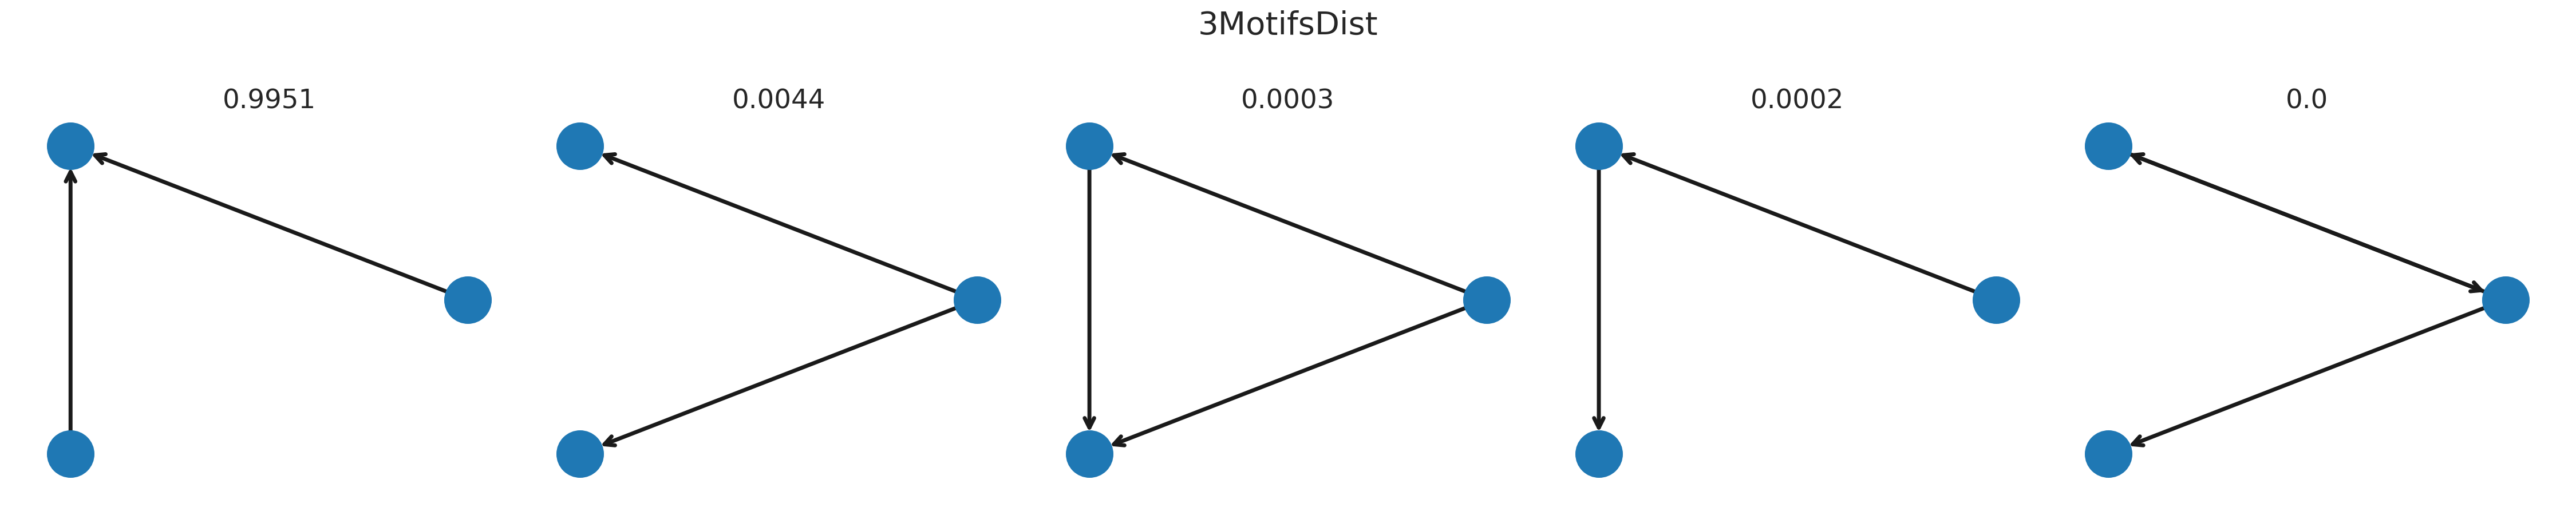
\includegraphics[width=\textwidth]{figures/swisscom/3motifs.png}
    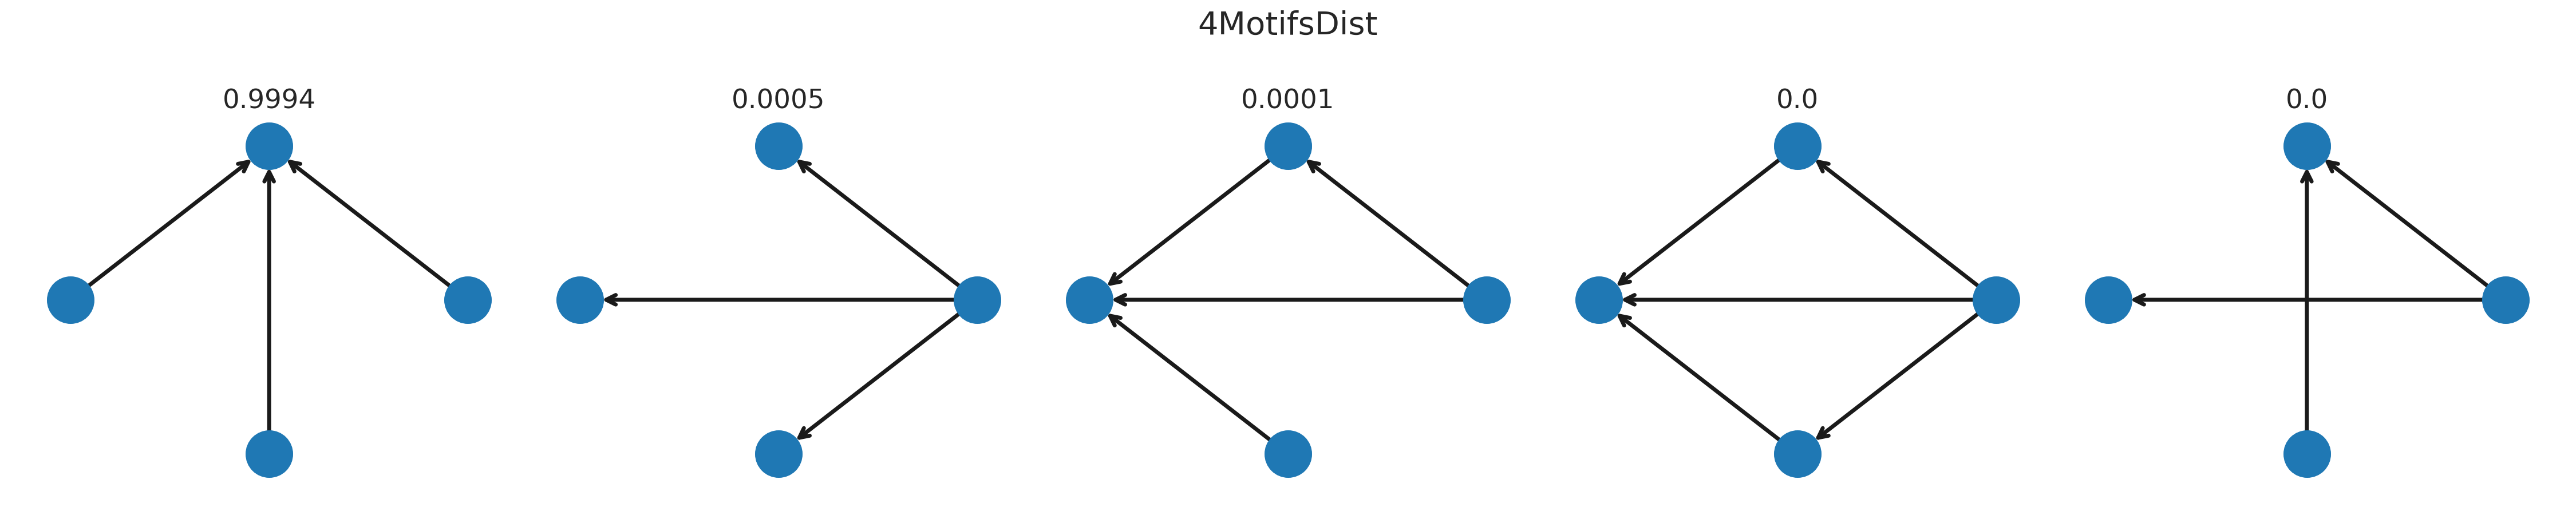
\includegraphics[width=\textwidth]{figures/swisscom/4motifs.png}
    \caption[Most common 5 structural motifs in Swisscom's internal knowledge graph and their frequencies.]{Most common 5 structural motifs in Swisscom's internal knowledge graph and their frequencies. Top vs bottom: 3-node vs 4-node motifs. Frequencies decrease from left to right.}
    \label{fig:motifs}
\end{figure}

\subsubsection{Summarization}

The KGist method was able to discover a meaningful summary of our knowledge graph. 10 association rules were returned and achieved a bit compression ratio of 68.45\% while explaining 96.10\% of the edges in the case of organization-rooted subgraph queries, while 7 returned rules achieved a bit compression ratio of 77.14\% while explaining 60.54\% of the edges in the case of site-rooted subgraph queries. Curiously, the method was not able to return a summary of any transport graph or the patent citation network. 

Unfortunately, the de-densification algorithm was not able to achieve substantial lossless compression, due to the already relatively low edge density of the Swisscom graph. Future work could consider a lossy version of the method or other potentially more powerful approaches. The spanning tree method identified prominent query paths for all graphs, where the distribution skewness for the Swisscom graph is in the medium range.

\subsubsection{Statistical tests}

We move on to presenting the results of our hypothesis testing. Table \ref{tab:pareto} reports which metrics for which datasets had a statistically significant probability of having a heavy-tailed distribution. We observe that this was proven true for the label distributions in the case of almost all datasets. In addition, interestingly, only for the Swisscom, transport, and citation cases, the motif frequencies are also heavy-tailed. Connected component sizes for a few datasets are significantly Pareto as well, though the Swisscom data is not among these cases.

\begin{table}[H]
    \centering
\caption[Pareto goodness of fit tests with p-values above a 0.05 significance threshold for knowledge graph datasets.]{Pareto goodness of fit tests with p-values (4th column) above a 0.05 significance threshold for knowledge graph datasets. For these metric distributions, we also report the estimated value of the polynomial degree parameter of the Pareto distribution (3rd column). For the 25 transport graphs, only the city with the highest p-value w.r.t. a metric is included for brevity.}
\label{tab:pareto}
% \begin{adjustbox}{width=0.75\columnwidth}
\begin{tabular}{llrr}
\toprule
             &                   &  $\alpha$ &  $p$ \\
Metric & Dataset &              &               \\
\midrule
WCC & transport-antofagasta &       0.0000 &        1.0000 \\
OverlappingRegionSizeDist & transport-bordeaux &       0.0000 &        1.0000 \\
RelationDist & redditHyperlinks &       0.0000 &        1.0000 \\
LabelInteractionDist & redditHyperlinks &       0.0000 &        1.0000 \\
NodeTypeDist & HepPh &       0.0000 &        1.0000 \\
RelationDist & HepPh &       0.0000 &        1.0000 \\
LabelInteractionDist & HepPh &       0.0000 &        1.0000 \\
NodeTypeDist & cit-Patents &       0.0000 &        1.0000 \\
RelationDist & cit-Patents &       0.0000 &        1.0000 \\
LabelInteractionDist & cit-Patents &       0.0000 &        1.0000 \\
             & transport-adelaide &       0.4572 &        1.0000 \\
NodeTypeDist & fb15k-237 &       0.0000 &        1.0000 \\
SCC & transport-palermo &       0.0000 &        1.0000 \\
RelationDist & transport-adelaide &       0.4572 &        1.0000 \\
NodeTypeDist & redditHyperlinks &       0.0000 &        1.0000 \\
             & transport-adelaide &       0.0000 &        1.0000 \\
             & ogbl-biokg &       2.2765 &        0.8730 \\
3MotifsDist & swisscom-big-orgs &       0.3522 &        0.7714 \\
             & swisscom-big-sites &       0.5061 &        0.7714 \\
             & transport-adelaide &       0.4454 &        0.7714 \\
WCC & fb15k-237 &       0.6184 &        0.4740 \\
             & ogbl-biokg &       0.5062 &        0.4740 \\
NodeTypeDist & wn18rr &       0.2397 &        0.3571 \\
3MotifsDist & cit-Patents &       0.6474 &        0.2286 \\
             & HepPh &       0.2362 &        0.0794 \\
NodeTypeDist & swisscom-big-sites &       0.2205 &        0.0530 \\
DisjointCommunitySizeDist & fb15k-237 &       0.8213 &        0.0314 \\
4MotifsDist & transport-belfast &       0.6811 &        0.0207 \\
NodeTypeDist & swisscom-big-orgs &       0.1042 &        0.0186 \\
\bottomrule
\end{tabular}
% \end{adjustbox}
\end{table}

Regarding the tests for metric uniformity across subgraphs, communities, and respective overlaps of the Swisscom data, the result is extremely positive, as all metric histograms appeared uniform with high statistical significance. 

Table \ref{tab:t} reports which metrics for which public datasets had a statistically significant probability of having equal distribution means with the metrics computed over Swisscom data. If for more than one public graph the p-value of the comparison was significant, we report the one with the largest p-value. 

Although for most metrics listed in this table, we discussed that for our graph, they are relatively different from what we observed for the public data, the t-test signals that there is at least no reason to reject the hypothesis of equal means. The negative sign of the statistic's values also supports our previous observations of commonly lower metric values for our graph. The results interestingly imply that at least some equivalence can be made between the Swisscom and public data w.r.t. the motif frequency, connected component size, or label distributions. The patent citation, WordNet, and transport networks stand out as examples.

\begin{table}[H]
    \centering
    \caption[Two-sample t-tests for metric distribution mean comparison between Swisscom and public data.]{Two-sample t-tests for metric distribution mean comparison between Swisscom and public data with p-values (5th column) above a 0.01 significance threshold. For these metric distribution pairs, we also report the estimated value of the t statistic (4th column). Only the public dataset with the highest p-value w.r.t. a metric is included for brevity.}
    \label{tab:t}
\begin{adjustbox}{width=0.85\columnwidth}
\begin{tabular}{lllrr}
\toprule
                   &                   &          &   $t$ &  $p$ \\
Dataset \#1 & Dataset \#2 & Metric &         &              \\
\midrule
swisscom-big-orgs & cit-Patents & 3MotifsDist &  0.0000 &       1.0000 \\
                   &                   & SCC &  0.0000 &       1.0000 \\
swisscom-big-sites & cit-Patents & SCC &  0.0000 &       1.0000 \\
swisscom-big-orgs & transport-belfast & 4MotifsDist & -0.0000 &       1.0000 \\
swisscom-big-sites & cit-Patents & 3MotifsDist &  0.0000 &       1.0000 \\
                   & transport-dublin & 4MotifsDist &  0.0000 &       1.0000 \\
                   & redditHyperlinks & WCC &  0.0784 &       0.9375 \\
                   & ogbl-biokg & BetweennessCentrality & -0.1708 &       0.8644 \\
                   & fb15k-237 & AuthorityScore & -0.2311 &       0.8172 \\
                   & wn18rr & NodeTypeDist & -0.3648 &       0.7263 \\
swisscom-big-orgs & redditHyperlinks & DisjointCommunitySizeDist & -0.3668 &       0.7138 \\
                   & wn18rr & RelationDist & -0.4231 &       0.6761 \\
swisscom-big-sites & ogbl-biokg & OverlappingCommunitySizeDist &  0.4250 &       0.6708 \\
swisscom-big-orgs & wn18rr & NodeTypeDist & -0.4403 &       0.6706 \\
                   & redditHyperlinks & WCC & -0.4682 &       0.6397 \\
swisscom-big-sites & wn18rr & RelationDist & -0.4920 &       0.6285 \\
swisscom-big-orgs & transport-helsinki & LabelInteractionDist & -0.8000 &       0.4645 \\
swisscom-big-sites & transport-helsinki & LabelInteractionDist & -0.8104 &       0.4611 \\
                   & redditHyperlinks & DisjointCommunitySizeDist &  0.7935 &       0.4276 \\
swisscom-big-orgs & cit-Patents & AuthorityScore & -0.8501 &       0.3953 \\
                   &                   & HubScore & -0.8828 &       0.3773 \\
                   & wn18rr & SpanningTreePathDist & -1.0341 &       0.3011 \\
swisscom-big-sites & cit-Patents & SpanningTreePathDist &  1.4331 &       0.1519 \\
                   & transport-belfast & HubScore & -1.4705 &       0.1416 \\
\bottomrule
\end{tabular}
\end{adjustbox}
\end{table}

On the other hand, Table \ref{tab:mmd} reports which metrics had a statistically significant probability of having equal distributions according to the Maximum Mean Discrepancy test. These results disprove a couple of the previous similarity insights; however, the label distribution similarity significance prevails, and now we also obtain the insight that the Swisscom graph's motif distribution is actually more similar to the NELL and transport graphs. The MMD test is more strict, but also more accurate, so we will assign greater value to these results compared to the Student tests.

Finally, no metrics had a statistically significant probability of having equal histogram means or low MMD across both query-based subgraphs and communities. Interestingly, both the query-based subgraphs and communities yield a highly representative partitioning of the big graph, though each is of its own nature. Respective overlapping regions, on the other hand, curiously had significant Student and MMD p-values only in the customer-site case, w.r.t. connected component size and graph diameter.

\begin{table}[H]
    \centering
        \caption[MMD tests for metric distribution comparison between Swisscom and public data.]{MMD tests for metric distribution comparison between Swisscom and public data with p-values (5th column) above a 0.01 significance threshold. For these metric distribution pairs, we also report the estimated value of the MMD statistic (4th column). Only the public dataset with the highest p-value w.r.t. a metric is included for brevity.}
    \label{tab:mmd}
\begin{adjustbox}{width=\columnwidth}
\begin{tabular}{lllrr}
\toprule
                   &           &                           &    MMD &  $p$ \\
Dataset \#1 & Dataset \#2 & Metric &        &            \\
\midrule
swisscom-big-orgs & transport-palermo & SCC & 0.0000 &     1.0000 \\
swisscom-big-sites & transport-antofagasta & 3MotifsDist & 0.0911 &     1.0000 \\
                   & transport-palermo & SCC & 0.0000 &     1.0000 \\
                   & transport-sydney & RelationDist & 0.0890 &     0.9500 \\
                   &           & LabelInteractionDist & 0.0902 &     0.8600 \\
swisscom-big-orgs & wn18rr & LabelInteractionDist & 0.0411 &     0.5800 \\
                   &           & NodeTypeDist & 0.1872 &     0.5400 \\
                   & transport-canberra & RelationDist & 0.3026 &     0.5100 \\
                   & nell-995 & 3MotifsDist & 0.1687 &     0.4300 \\
swisscom-big-sites & transport-sydney & NodeTypeDist & 1.4733 &     0.3300 \\
                   &           & WCC & 0.0420 &     0.2500 \\
swisscom-big-orgs & ogbl-biokg & WCC & 0.1441 &     0.2400 \\
swisscom-big-sites & nell-995 & 4MotifsDist & 0.0494 &     0.2300 \\
swisscom-big-orgs & fb15k-237 & 4MotifsDist & 0.1081 &     0.0900 \\
swisscom-big-sites & fb15k-237 & DisjointCommunitySizeDist & 0.1601 &     0.0200 \\
\bottomrule
\end{tabular}
\end{adjustbox}
\end{table}

\subsubsection{Reasoning experiments for Monty}

To finalize the result discussion, we provide in Table \ref{tab:swisscom_coins} the achieved knowledge graph reasoning results after applying COINs to Monty data. Query answering experiments were focused on single-hop queries only, as a proof of concept. A train-validation-test data split of the Monty data was obtained through uniform stratified sampling, while COIN's hyperparameters were set to the same values as for the WN18RR dataset (this is supported by the previous discussion indicating the similarity between these two graphs). 

We observe how the Swisscom metrics are in about the same range as those achieved on the academic data, implying we have obtained an approach that successfully generalizes. In addition, when estimating the scalability benefits of COINs for Monty, we obtained that \emph{728.7} times fewer query embeddings were computed during evaluation, and \emph{228.36} times less training memory was used in comparison to the baseline, proving that COINs' benefits can indeed scale with graph size.


\begin{table}[H]
    \centering
    \caption[Link prediction and query answering metrics after applying COINs-modified models to the Swisscom dataset.]{Link prediction and query answering metrics after applying COINs-modified models to the Swisscom dataset (higher is better), with a comparison to the best results of the same models on the academic knowledge graphs. The best value per metric is highlighted in bold.}
    \label{tab:swisscom_coins}
    % \begin{adjustbox}{width=0.75\columnwidth}
    \begin{tabular}{llrrrrrr}
    \toprule
         Dataset & Model & F1 & AP & Hits@1 & Hits@3 & Hits@10 & MRR \\
    \midrule
         FB15k-237 & COINs-Best & 0.938 & 0.900 & 0.333 & 0.477 & 0.626 & 0.431 \\
         WN18RR & COINs-Best & 0.917 & 0.871 & 0.436 & 0.510 & 0.586 & 0.487 \\
         NELL-995 & COINs-Best & 0.965 & 0.963 & 0.445 & 0.633 & 0.740 & 0.555 \\
         \midrule
         Monty & COINs-TransE & 0.875 & \textbf{0.749} & 0.048 & 0.159 & 0.334 & 0.138 \\
         Monty & COINs-DistMult & \textbf{0.893} & 0.740 & 0.165 & 0.241 & 0.343 & 0.223 \\
         Monty & COINs-ComplEx & 0.889 & 0.736 & \textbf{0.428} & \textbf{0.446} & \textbf{0.459} & \textbf{0.441} \\
         Monty & COINs-RotatE & 0.719 & 0.554 & \textbf{0.428} & 0.444 & 0.452 & 0.439 \\
    \bottomrule
    \end{tabular}
    % \end{adjustbox}
\end{table}

\subsection{Summary}
\label{sec:summary}

In this section, we have presented a detailed descriptive and comparative knowledge graph analysis methodology that was applied for data collected for diagnostic purposes in the telecommunications sector, though it is general and detailed so as to be operationalized for broader research purposes. We dissected a knowledge graph with five classes of network science measuring techniques and utilized one-sample goodness of fit and two-sample distribution comparison statistical tests to quantitatively analyze the obtained measures.

The obtained results yielded a plethora of non-trivial insights into our data source, from which the main conclusion one can extract is that the Swisscom data is more similar to knowledge graph datasets traditionally constructed for learning knowledge graph reasoning than to random graphs like citation networks. This paves the way for future research at the company in improving the current query answering model trained on this data. Before us is thus another instance of a mixture between holistic and reductionist views of a knowledge graph that could not provide the same value on their own.
